
\documentclass[11pt,a4paper]{article}
\usepackage{ucs}
\usepackage[utf8x]{inputenc}
\usepackage[T1]{fontenc}
\usepackage{ngerman}
\usepackage{amsmath,amssymb,amstext}
\usepackage{tikz}
\title{Rechnerstrukturen Blatt 3}
\author{Sven Marquardt}
\date{\today}
%% This is file `kvmacros.tex',
%% Version of January 7th, 2002
%% 
%% Copyright (C) 1998-2002 by Andreas W. Wieland, awwieland@gmx.de 
%%
%% This program can be redistributed and/or modified under the terms
%% of the LaTeX Project Public License distributed from CTAN
%% archives in directory macros/latex/base/lppl.txt; either
%% version 1 of the License, or (at your option) any later version,
%% with `The Program' referring to the software `kvmacros.tex' and its
%% accompanying documentation and `The Copyright Holder' referring to the
%% person Andreas W. Wieland.
%% 
%% 
%% 
%% IMPORTANT NOTICE: 
%% 
%% For error reports, comments or suggestions in case of UNCHANGED 
%% versions send mail to:
%% awwieland@gmx.de
%% 
%% Anyway, if you use my macros, send me an eMail, too. I would like to know
%% if they are useful to somebody out there.
%%
%% Please do not request updates from me directly. Distribution is 
%% done through Mail-Servers and TeX organizations. 
%% 
%% You are allowed to distribute this file under the condition that 
%% it is distributed together with `kvdoc.tex', `kvdoc.dvi' and `kvdoc.ps'. 
%% 
%% If you receive this file alone from someone, complain! 
%%
\typeout{}
\typeout{Macros for typesetting Karnaugh maps and Veitch charts}
\typeout{Version of January 7th, 2002}
\typeout{by Andreas W. Wieland, awwieland@gmx.de}
\typeout{}
%%
%% Change History:
%% August 04th, 1998: Original Version
%%
%% August 19th, 1998: Minor changes to make the lines within the maps look
%% better, also moved the variable identifiers from the right to the left and
%% added an identifier for the logic function; since then \kvmap has 5
%% instead of 4 parameters. I also included the documentation in an additional
%% Postscript-file.  
%%
%% September 23rd, 1998: Fixed the problem with double braces by introducing
%% the \compdummy and \ende macros in the \ifx-comparisons (see below): 
%% The parameters that are longer than one character do not have to be
%% enclosed in double braces any longer --- single braces are
%% sufficient. However, double braces will still be processed correctly.
%%
%% May 19th, 1999: Changed the documentation (which was months overdue) after
%% F. M. Brown pointed me to the incorrectness of the term
%% "Karnaugh-Veitch-map". Actually, the macros itself haven't
%% changed. Probably I should introduce macros for typesetting Veitch charts
%% as well (which would be a minor task). This version was actually never
%% released. 
%%
%% May 25th, 1999: Introduced macros for Veitch charts
%% (\veitchfoo) and renamed the macros that are solely related to
%% Karnaugh maps from \kvfoo to \karnaughfoo. Introduced aliases for those
%% macros that are user-callable to maintain compatibility with older versions:
%% \kvmap -> \karnaughmap. However, \kvindex, \kvnoindex and \kvunitlength
%% haven't changed their names as they are related to both Karnaugh maps and
%% Veitch charts. Changed the (plain stupid) algorithm that processes the
%% variable-length arguments so that it takes much less time to produce large
%% maps. Several macros so became redundant and are no longer included. Also I
%% introduced \kvindexsize and \kvcontentsize to adjust the font size of the
%% indices and the contents of a diagram. They default to \tiny and
%% \normalsize. 
%%
%% January 17th, 2001: Changed the eMail-address in the macro file and the
%% accompanying documentation and made minor changes to the documentation.
%%
%% January 7th, 2002: Exchanged the \xdef to \gdef in the definition of
%% \kvargumentstring and \kvgetonechar so that things like {\textbf 1} in the
%% argumentlist of \karnaughmap do not cause error messages any longer. 
%% Thanks to Michal Medveck{\'y} for pointing me to this error.
%%
%%
%%
%% We need a fixed dimension for a single field in a Karnaugh map:
%%
\newdimen\kvunitlength
\kvunitlength=8mm
%%
%% We need a default font size for the indices:
%%
\newcommand{\kvindexsize}{\tiny}
%%
%% And we need a default size for the contents and variable identifiers:
%%
\newcommand{\kvcontentsize}{\normalsize}
%%
%% First, we have to introduce some counters:
%%
%% \kvrecursiondepth is used to control the recursion of the
%% \karnaughmakemap- and \veitchmakechart-macro. 
%%
\newcount\kvrecursiondepth
%%
%% The \kvindexcounter is needed for the indices in the fields of the
%% diagrams. 
%%
\newcount\kvindexcounter
%% 
%% \kvxsize and \kvysize store the dimensions of an entire diagram.
%%
\newcount\kvxsize
\newcount\kvysize
%%
%% Some counters are necessary to compute the marks for the variable
%% identifiers:
%%
\newcount\kvvarno
\newcount\kvxvarno
\newcount\kvyvarno
\newcount\kvmarkstart
\newcount\kvmarklength
\newcount\kvmarknum
\newcount\kvmarkmove
%%
%% And we need a savebox to store the variable marks:
%%
\newsavebox\kvsavebox
%%
%% Single fields in a diagram should be indexed, which makes the map easier to
%% use. This is the default. If you don't want indices, simply call
%% \kvnoindex. If you want indices back, call \kvindex:
%%
\def\kvnoindex{%
\def\kvcurrentindex{}}
%%
\def\kvindex{%
\def\kvcurrentindex{%
\the\kvindexcounter\global\advance\kvindexcounter by 1}%
}
%%
\kvindex
%%
%% We need a macro that computes the powers of two:
%%
\def\kvpoweroftwo#1#2{% Computes #1=2^#2, both of which have to be counters
{\ifnum#2>0 
\global\multiply#1 by 2 
\advance#2 by -1
\kvpoweroftwo{#1}{#2}
\fi}}
%%
%% The macros \kvargumentstring, \kvgetchar and \kvgetonechar are needed to
%% process the variabe-length parameters in \karnaughmap and \veitchchart:
%%
\def\kvargumentstring#1{\gdef\kvdummystring{#1{}\noexpand\end}}
%%
\def\kvgetchar{\expandafter\kvgetonechar\kvdummystring}
%%
\def\kvgetonechar#1#2\end{{#1}\gdef\kvdummystring{#2\noexpand\end}}%
%%
%% The Macro \karnaughmakemap calls itself recursively until the parameter #1
%% equals 1, whereupon it returns a single token from the list of arguments,
%% enclosed in a \makebox plus the index (if enabled) in a smaller \makebox:
%%
\def\karnaughmakemap#1#2{{%
\kvrecursiondepth=\number#1
\ifnum\kvrecursiondepth>1
\divide\kvrecursiondepth by 2
\unitlength=\kvunitlength
\multiply\unitlength by \kvrecursiondepth
%%
\ifcase#2
%%
%% The parameter #2 of \karnaughmakemap is needed because the inner Karnaugh
%% maps need to be mirrored. This is achieved by the following case-statement,
%% which orders the inner Karnaugh maps properly:
%%
%% Case 0: top-left Karnaugh map
\begin{picture}(2,2)%
\put(0,1){\karnaughmakemap{\kvrecursiondepth}{0}}%
\put(1,1){\karnaughmakemap{\kvrecursiondepth}{1}}%
\put(0,0){\karnaughmakemap{\kvrecursiondepth}{2}}%
\put(1,0){\karnaughmakemap{\kvrecursiondepth}{3}}%
\end{picture}%
\or
%% Case 1: top-right Karnaugh map
\begin{picture}(2,2)%
\put(1,1){\karnaughmakemap{\kvrecursiondepth}{1}}%
\put(0,1){\karnaughmakemap{\kvrecursiondepth}{0}}%
\put(1,0){\karnaughmakemap{\kvrecursiondepth}{3}}%
\put(0,0){\karnaughmakemap{\kvrecursiondepth}{2}}%
\end{picture}%
\or
%% Case 2: bottom-left Karnaugh map
\begin{picture}(2,2)%
\put(0,0){\karnaughmakemap{\kvrecursiondepth}{2}}%
\put(1,0){\karnaughmakemap{\kvrecursiondepth}{3}}%
\put(0,1){\karnaughmakemap{\kvrecursiondepth}{0}}%
\put(1,1){\karnaughmakemap{\kvrecursiondepth}{1}}%
\end{picture}%
\or
%% Case 3: bottom-right Karnaugh map
\begin{picture}(2,2)%
\put(1,0){\karnaughmakemap{\kvrecursiondepth}{3}}%
\put(0,0){\karnaughmakemap{\kvrecursiondepth}{2}}%
\put(1,1){\karnaughmakemap{\kvrecursiondepth}{1}}%
\put(0,1){\karnaughmakemap{\kvrecursiondepth}{0}}%
\end{picture}%
\fi
\else
\unitlength=\kvunitlength
\begin{picture}(1,1)
\put(0,0){\makebox(1,1){\kvcontentsize\kvgetchar}}%
\put(0.05,0.05){\makebox(0.9,0.9)[bl]{\kvindexsize\kvcurrentindex}}%
\end{picture}
\fi}}%
%%
%% \karnaughmaketopmark typesets the variable marks of a Karnaugh map that are
%% located on top of the diagram:
%%
\def\karnaughmaketopmark{%
  \unitlength\kvunitlength
  \begin{picture}(\kvxsize,1)
    \kvmarkstart=1
    \kvpoweroftwo{\kvmarkstart}{\kvxvarno} % \kvymarkstart is the start 
                                % position for the \multiput
    \kvmarklength=\kvmarkstart 
    \multiply\kvmarklength by 2 % \kvmarklength is the length of a mark
    \kvmarkmove=\kvmarkstart 
    \multiply\kvmarkmove by 4 % This is the move distance for the \multiput.
    \kvmarknum=\kvxsize
    \divide\kvmarknum by \kvmarkmove % This is the number of repetitions for
                                % the \multiput.  
    %The highest-order variable mark needs a special treatment:
    \ifnum\kvmarknum=0\kvmarknum=1\divide\kvmarklength by 2\fi 
    \savebox\kvsavebox(\kvmarklength,1){% 
      \begin{picture}(\kvmarklength,1)
      \put(0,0.3){\makebox(\kvmarklength,0.7){\kvcontentsize\kvgetchar}} 
      \put(0,0.1){\line(0,1){0.4}} 
      \put(\kvmarklength,0.1){\line(0,1){0.4}}
      \put(0,0.3){\line(1,0){\kvmarklength}} 
      \end{picture}}
    \multiput(\kvmarkstart,0)(\kvmarkmove,0){\kvmarknum}{\usebox\kvsavebox}
  \end{picture}
}
%%
%% \karnaughmakeleftmark typesets the variable marks of a Karnaugh map that are
%% located on the left of the diagram:
%%
\def\karnaughmakeleftmark{%
  \unitlength\kvunitlength
  \begin{picture}(-1,\kvysize)(0,-\kvysize)
    \kvmarkstart=1
    \kvpoweroftwo{\kvmarkstart}{\kvyvarno} % \kvmarkstart is the start 
                                % position for the \multiput
    \kvmarklength=\kvmarkstart 
    \multiply\kvmarklength by 2 % \kvmarklength is the length of a mark
    \kvmarkmove=\kvmarkstart 
    \multiply\kvmarkmove by 4 % This now is the move distance for the
                              % \multiput. 
    \kvmarknum=\kvysize
    \divide\kvmarknum by \kvmarkmove % This now is the number of 
                                % repetitions for the \multiput.  
    %The highest-order variable mark needs a special treatment:
    \ifnum\kvmarknum=0\kvmarknum=1\divide\kvmarklength by 2\fi 
    \advance\kvmarkstart by \kvmarklength
    \savebox\kvsavebox(1,\kvmarklength){%
      \begin{picture}(1,\kvmarklength)
        \put(-0.3,0){\makebox(-0.7,\kvmarklength){\kvcontentsize\kvgetchar}}
        \put(-0.1,0){\line(-1,0){0.4}}
        \put(-0.1,\kvmarklength){\line(-1,0){0.4}}
        \put(-0.3,0){\line(0,1){\kvmarklength}}
      \end{picture}}
    \multiput(0,-\kvmarkstart)(0,-\kvmarkmove){\kvmarknum}{\usebox\kvsavebox}
  \end{picture}
}
%% \karnaughmakemarks calls \karnaughmaketopmark or \karnaughmakeleftmark
%% depending on whether \kvvarno is odd or even.
%%
\def\karnaughmakemarks{%
\ifnum\kvvarno>0
  \let\next=\karnaughmakemarks
  \ifodd\kvvarno % We have to make a mark at the top
    \advance\kvxvarno by -1
    \put(0,\kvxvarno){\karnaughmaketopmark}
  \else % We have to make a mark at the left
    \advance\kvyvarno by -1
    \put(-\kvyvarno,-\kvysize){\karnaughmakeleftmark}
  \fi
  \advance\kvvarno by -1
\else
  \let\next=\relax
\fi
\next
}
%%
%% \karnaughmap is the macro that a user calls if he wants to draw a
%% Karnaugh map:  
%%
\def\karnaughmap#1#2#3#4#5{%
%%
%% #1 is the number of variables in the Karnaugh map
%% #2 is the identifier of the function
%% #3 is the list of identifiers of those variables 
%% #4 is the list of tokens that have to be written into the map
%% #5 is something that you want to draw inside the Karnaugh map
%%
\kvvarno=#1  % \kvvarno is the total number of variables 
\kvyvarno=#1 % \kvyvarno is the number of variable marks at the left 
\divide\kvyvarno by 2
\kvxvarno=#1 % \kvxvarno is the number of variable marks on top 
\advance\kvxvarno by -\kvyvarno
\kvxsize=1
\kvpoweroftwo{\kvxsize}{\kvxvarno}
\kvysize=1
\kvpoweroftwo{\kvysize}{\kvyvarno}
\advance\kvxsize by \kvyvarno
\advance\kvxvarno by \kvysize
\unitlength\kvunitlength
\begin{picture}(\kvxsize,\kvxvarno)(-\kvyvarno,-\kvysize)
\advance\kvxsize by -\kvyvarno
\advance\kvxvarno by -\kvysize
\put(0,-\kvysize){%
\begin{picture}(\kvxsize,\kvysize)
\multiput(0,0)(0,1){\kvysize}{\line(1,0){\kvxsize}}
\multiput(0,0)(1,0){\kvxsize}{\line(0,1){\kvysize}}
\put(0,\kvysize){\line(1,0){\kvxsize}}
\put(\kvxsize,0){\line(0,1){\kvysize}}
#5
\end{picture}}
\put(-\kvyvarno,0){\makebox(\kvyvarno,\kvxvarno){#2}}
\kvindexcounter=0
\kvargumentstring{#4}
\put(0,-\kvysize){\karnaughmakemap{\kvysize}{0}}
\ifodd\kvvarno
{\divide\kvxsize by 2
\put(\kvxsize,-\kvysize){\karnaughmakemap{\kvysize}{1}}}
\fi
\kvargumentstring{#3}
\karnaughmakemarks
%%
\end{picture}
}%
%%
%% The definition of \kvmap is necessary to maintain compatibility with older
%% versions of this macro package:
%%
\def\kvmap{\karnaughmap}%
%%
%%
%% The Macro \veitchmakechart calls itself recursively until the parameter #1
%% equals 1, whereupon it returns a single token from the list of arguments,
%% enclosed in a \makebox plus the index (if enabled) in a smaller \makebox:
%%
\def\veitchmakechart#1{{%
\kvrecursiondepth=\number#1
\ifnum\kvrecursiondepth>1
\divide\kvrecursiondepth by 2
\unitlength=\kvunitlength
\multiply\unitlength by \kvrecursiondepth
%%
\begin{picture}(2,2)%
\put(0,1){\veitchmakechart{\kvrecursiondepth}}%
\put(1,1){\veitchmakechart{\kvrecursiondepth}}%
\put(0,0){\veitchmakechart{\kvrecursiondepth}}%
\put(1,0){\veitchmakechart{\kvrecursiondepth}}%
\end{picture}%
\else
\unitlength=\kvunitlength
\begin{picture}(1,1)
\put(0,0){\makebox(1,1){\kvcontentsize\kvgetchar}}%
\put(0.05,0.05){\makebox(0.9,0.9)[bl]{\kvindexsize\kvcurrentindex}}%
\end{picture}
\fi}}%
%%
\def\veitchmaketopmark{%
  \unitlength\kvunitlength
  \begin{picture}(\kvxsize,1)
    \kvmarkstart=1
    \kvpoweroftwo{\kvmarkstart}{\kvxvarno} % \kvymarkstart is the start 
                                % position for the \multiput
    \kvmarklength=\kvmarkstart % \kvmarklength is the length of a mark
    \kvmarkmove=\kvmarkstart 
    \multiply\kvmarkmove by 2 % This is the move distance for the \multiput.
    \kvmarknum=\kvxsize
    \divide\kvmarknum by \kvmarkmove % This is the number of repetitions for
                                     % the \multiput.  
    \savebox\kvsavebox(\kvmarklength,1){% 
      \begin{picture}(\kvmarklength,1)
      \put(0,0.3){\makebox(\kvmarklength,0.7){\kvcontentsize\kvgetchar}} 
      \put(0,0.1){\line(0,1){0.4}} 
      \put(\kvmarklength,0.1){\line(0,1){0.4}}
      \put(0,0.3){\line(1,0){\kvmarklength}} 
      \end{picture}}
    \multiput(\kvmarkstart,0)(\kvmarkmove,0){\kvmarknum}{\usebox\kvsavebox}
  \end{picture}
}
%%
\def\veitchmakeleftmark{%
  \unitlength\kvunitlength
  \begin{picture}(-1,\kvysize)(0,-\kvysize)
    \kvmarkstart=1
    \kvpoweroftwo{\kvmarkstart}{\kvyvarno} % \kvmarkstart is the start 
                                % position for the \multiput
    \kvmarklength=\kvmarkstart 
    \kvmarkmove=\kvmarkstart 
    \multiply\kvmarkmove by 2 % This now is the move distance for the \multiput. 
    \kvmarknum=\kvysize
    \divide\kvmarknum by \kvmarkmove % This now is the number of 
                                     % repetitions for the \multiput.  
    \advance\kvmarkstart by \kvmarklength
    \savebox\kvsavebox(1,\kvmarklength){%
      \begin{picture}(1,\kvmarklength)
        \put(-0.3,0){\makebox(-0.7,\kvmarklength){\kvcontentsize\kvgetchar}}
        \put(-0.1,0){\line(-1,0){0.4}}
        \put(-0.1,\kvmarklength){\line(-1,0){0.4}}
        \put(-0.3,0){\line(0,1){\kvmarklength}}
      \end{picture}}
    \multiput(0,-\kvmarkstart)(0,-\kvmarkmove){\kvmarknum}{\usebox\kvsavebox}
  \end{picture}
}
%%
\def\veitchmakemarks{%
\ifnum\kvvarno>0
  \let\next=\veitchmakemarks
  \ifodd\kvvarno % We have to make a mark at the top
    \advance\kvxvarno by -1
    \put(0,\kvxvarno){\veitchmaketopmark}
  \else % We have to make a mark at the left
    \advance\kvyvarno by -1
    \put(-\kvyvarno,-\kvysize){\veitchmakeleftmark}
  \fi
  \advance\kvvarno by -1
\else
  \let\next=\relax
\fi
\next
}
%%
\def\veitchchart#1#2#3#4#5{%
%%
%% #1 is the number of variables in the Veitch chart
%% #2 is the identifier of the function
%% #3 is the list of identifiers of those variables 
%% #4 is the list of tokens that have to be written into the chart
%% #5 is something that you want to draw inside the Veitch chart
%%
\kvvarno=#1  % \kvvarno is the total number of variables 
\kvyvarno=#1 % \kvyvarno is the number of variable marks at the left 
\divide\kvyvarno by 2
\kvxvarno=#1 % \kvxvarno is the number of variable marks on top 
\advance\kvxvarno by -\kvyvarno
\kvxsize=1
\kvpoweroftwo{\kvxsize}{\kvxvarno}
\kvysize=1
\kvpoweroftwo{\kvysize}{\kvyvarno}
\advance\kvxsize by \kvyvarno
\advance\kvxvarno by \kvysize
\unitlength\kvunitlength
\begin{picture}(\kvxsize,\kvxvarno)(-\kvyvarno,-\kvysize)
\advance\kvxsize by -\kvyvarno
\advance\kvxvarno by -\kvysize
\put(0,-\kvysize){%
\begin{picture}(\kvxsize,\kvysize)
\multiput(0,0)(0,1){\kvysize}{\line(1,0){\kvxsize}}
\multiput(0,0)(1,0){\kvxsize}{\line(0,1){\kvysize}}
\put(0,\kvysize){\line(1,0){\kvxsize}}
\put(\kvxsize,0){\line(0,1){\kvysize}}
#5
\end{picture}}
\put(-\kvyvarno,0){\makebox(\kvyvarno,\kvxvarno){#2}}
\kvindexcounter=0
\kvargumentstring{#4}
\put(0,-\kvysize){\veitchmakechart{\kvysize}}
\ifodd\kvvarno
{\divide\kvxsize by 2
\put(\kvxsize,-\kvysize){\veitchmakechart{\kvysize}}}
\fi
\kvargumentstring{#3}
\veitchmakemarks
%%
\end{picture}
}%
%%

%%% Local Variables: 
%%% mode: latex
%%% TeX-master: t
%%% End: 

\usetikzlibrary{automata}
\usetikzlibrary{positioning}
\usetikzlibrary{topaths}
\begin{document}
Aufgabe3.1\\
Die Schaltung soll einen Zähler darstellen, der in 3er Schritten vorwärts oder rückwärts zählt. Das Umstellen der Zählrichtung erfolgt durch den Schalter $x_0$.\\
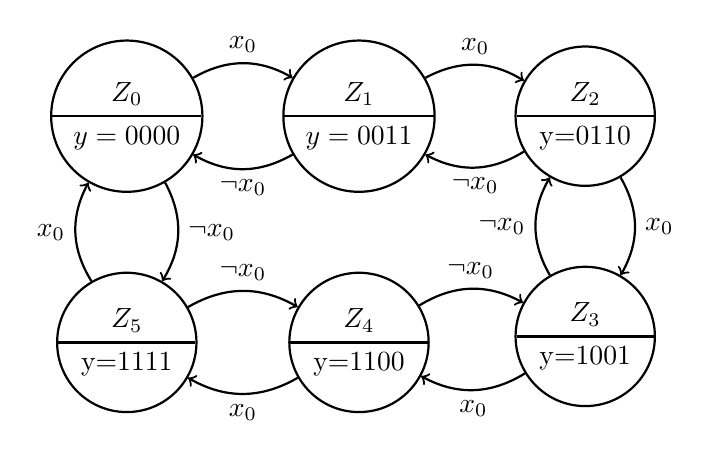
\begin{tikzpicture}[auto,thick]
	\node[state with output] (Z0) {$Z_0$ \nodepart {lower} $y=0000$};
	\node[state with output, right=of Z0] (Z1) {$Z_1$ \nodepart {lower} $y=0011$};
	\node[state with output, right=of Z1] (Z2) {$Z_2$ \nodepart {lower} y=0110};
	\node[state with output, below=of Z2] (Z3) {$Z_3$ \nodepart {lower} y=1001};
	\node[state with output, below=of Z1] (Z4) {$Z_4$ \nodepart {lower} y=1100};
	\node[state with output, below=of Z0] (Z5) {$Z_5$ \nodepart {lower} y=1111};
	\path[->] (Z0)	edge [bend left]		node	{$x_0$}(Z1)
			  		edge [bend left]		node[right]	{$\neg x_0$}(Z5)
			  (Z1)	edge [bend left]		node	{$\neg x_0$}(Z0)
			  		edge [bend left]		node	{$x_0$}(Z2)
			  (Z2)	edge [bend left]		node	{$\neg x_0$}(Z1)
			  		edge [bend left]		node	{$x_0$}(Z3)
			  (Z3)	edge [bend left]		node	{$\neg x_0$}(Z2)
			  		edge [bend left]		node	{$x_0$}(Z4)
			  (Z4)	edge [bend left]		node	{$\neg x_0$}(Z3)
			  		edge [bend left]		node	{$x_0$}(Z5)
			  (Z5)	edge [bend left]		node[left]	{$x_0$}(Z0)			  		
			  		edge [bend left]		node	{$\neg x_0$}(Z4);
\end{tikzpicture}
\\
A=$ ( X,Y,Z, \delta, \mu ) $ ,mit\\
$X= \lbrace 0,1 \rbrace$\\
$Y= \lbrace 0000,0011,0110,1001,1100,1111 \rbrace$\\
$Z= \lbrace 000,001,010,011,100,101 \rbrace$\\
$\delta : Z \times X \rightarrow Z$\\
$\mu : Z \rightarrow Y$\\ \\
Dazu die Wertetabelle \\ \\
\begin{tabular}{c | c | c | c | c | | c | c | c | c | | c | c | c | c}
$x_0$&Z&$z_2$&$z_1$&$z_0$&$y_3$&$y_2$&$y_1$&$y_0$&$Z^+$&$z^+_2$&$z^+_1$&$z^+_0$ \\ \hline
0&$Z_0$&0&0&0&0&0&0&0&$Z_1$&0&0&1\\
0&$Z_1$&0&0&1&0&0&1&1&$Z_2$&0&1&0\\
0&$Z_2$&0&1&0&0&1&1&0&$Z_3$&0&1&1\\
0&$Z_3$&0&1&1&1&0&0&1&$Z_4$&1&0&0\\
0&$Z_4$&1&0&0&1&1&0&0&$Z_5$&1&0&1\\
0&$Z_5$&1&0&1&1&1&1&1&$Z_0$&0&0&0\\
0&--&1&1&0&*&*&*&*&--&*&*&*\\
0&--&1&1&1&*&*&*&*&--&*&*&*\\ \hline
1&$Z_0$&0&0&0&0&0&0&0&$Z_5$&1&0&1\\
1&$Z_1$&0&0&1&0&0&1&1&$Z_0$&0&0&0\\
1&$Z_2$&0&1&0&0&1&1&0&$Z_1$&0&0&1\\
1&$Z_3$&0&1&1&1&0&0&1&$Z_2$&0&1&0\\
1&$Z_4$&1&0&0&1&1&0&0&$Z_3$&0&1&1\\
1&$Z_5$&1&0&1&1&1&1&1&$Z_4$&1&0&0\\
1&--&1&1&0&*&*&*&*&--&*&*&*\\
1&--&1&1&1&*&*&*&*&--&*&*&*\\
\end{tabular}\\
\\ \\  \\
Daraus ergeben sich folgende KV-Diagramme für $z^+_2,z^+_1$ und $z^+_0$.\\
\karnaughmap{4}{$z^+_2$}{{$x_0$}{$z_2$}{$z_1$}{$z_0$}}{000110**100001**}{
\textcolor{blue}{
\put(3.5,3){\oval(1.0,1.9)[]}}
\textcolor{red}{
\put(1.85,2.5){\oval(1.9,1.0)[]}}
\textcolor{black}{
\put(0.2,0.5){\oval(1.0,1.0)[]}}
\textcolor{green}{
\put(2,1){\oval(1.0,1.9)[]}}
}\\
$z^+_2=\textcolor{blue}{ (\neg z_0 \wedge z_2 \wedge \neg x_0 ) } \vee \textcolor{red}{(z_0 \wedge z_1 \wedge \neg x_0)} \vee \textcolor{green}{(z_0 \wedge z_2 \wedge x_0)} \vee \textcolor{black}{ ( \neg z_0 \wedge \neg z_1 \wedge \neg z_2 \wedge x_0)}$\\
\karnaughmap{4}{$z^+_1$}{{$x_0$}{$z_2$}{$z_1$}{$z_0$}}{011000**000101**}{
\textcolor{red}{
\put(1.5,3.5){\oval(1.0,1.0)[]}
}
\textcolor{blue}{
\put(-0.15,2.5){\oval(1.8,0.9)[r]}
\put(3.85,2.5){\oval(1.8,0.9)[l]}
}
\textcolor{green}{
\put(1.7,1.5){\oval(1.9,0.9)[]}}
\textcolor{black}{
\put(2,1){\oval(0.9,1.9)[]}}
}\\
$z^+_1= \textcolor{red}{(z_0 \wedge \neg z_1 \wedge \neg z_2 \wedge \neg x_0)} \vee \textcolor{blue}{(\neg z_0 \wedge z_1 \wedge \neg x_0)} \vee \textcolor{green}{(z_0 \wedge z_1 \wedge x_0)} \vee (z_0 \wedge z_2 \wedge x_0)$\\
\karnaughmap{4}{$z^+_0$}{{$x_0$}{$z_2$}{$z_1$}{$z_0$}}{101010**101010**}{
\textcolor{red}{
\put(-0.04,1.95){\oval(2,3.9)[r]}
\put(4.04,1.95){\oval(2.01,3.9)[l]}
}
}
$z^+_0=\textcolor{red}{\neg z_0}$\\ 
Folglich bilden folgende KV-Diagramme die Minimierung der Ausgangsfunktion.\\
\kvunitlength=5mm
\karnaughmap{3}{$y_3$}{{$z_2$}{$z_1$}{$z_0$}}{000111**}{
\textcolor{red}{
\put(3,1){\oval(2,2)}}
\textcolor{blue}{
\put(1.85,0.5){\oval(2,1)}}
}
$y_3= \textcolor{red}{z_2} \vee \textcolor{blue}{(z_0 \wedge z_1)}$
\karnaughmap{3}{$y_2$}{{$z_2$}{$z_1$}{$z_0$}}{001011**}{
\textcolor{red}{
\put(3,1){\oval(2,2)}}
\textcolor{blue}{
\put(-0.15,0.5){\oval(2,0.9)[r]}
\put(3.85,0.5){\oval(2,0.9)[l]}}
}
$y_2= \textcolor{red}{z_2} \vee \textcolor{blue}{ ( \neg z_0 \wedge z_1)}$\\
\karnaughmap{3}{$y_1$}{{$z_2$}{$z_1$}{$z_0$}}{011001**}{
\textcolor{red}{
\put(2,1.5){\oval(2,1)}}
\textcolor{blue}{
\put(-0.15,0.5){\oval(2,0.9)[r]}
\put(3.85,0.5){\oval(2,0.9)[l]}}}
$y_1=\textcolor{red}{(z_0 \wedge \neg z_1)} \vee \textcolor{blue}{(\neg z_0 \wedge z_1)}$
\karnaughmap{3}{$y_0$}{{$z_2$}{$z_1$}{$z_0$}}{010101**}{
\textcolor{red}{
\put(2,1){\oval(2,2)}}}
$y_0=\textcolor{red}{z_0}$\\ \\ \\

Aufgabe 3.2\\
In dieser Aufgabe soll eine Ampel implementiert werden, die automatisch läuft. Heißt, nach einer gewissen Zeit gibt es automatisch Grün für die Fußgänger, ohne dass ein Knopf gedrückt werden muss. Es ist also ein autonomer Automat. Folglich beschreibt folgender Automat die Funktion der Ampel. \\
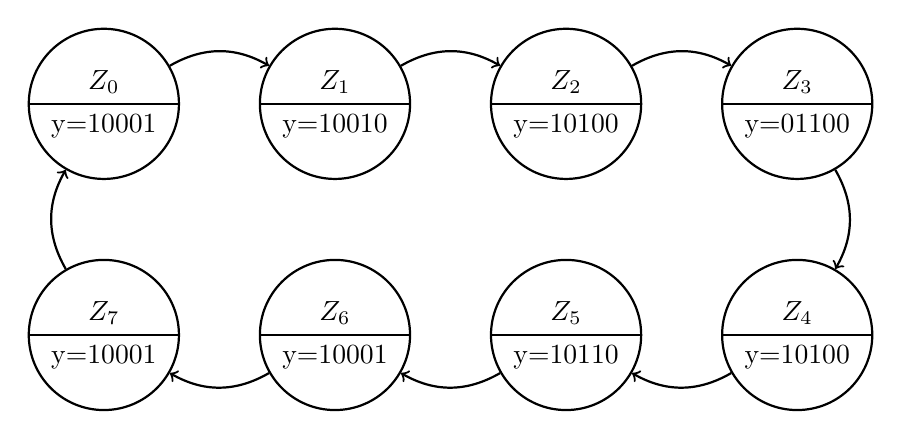
\begin{tikzpicture}[auto,thick]
	\node[state with output] (Z0) {$Z_0$ \nodepart {lower} y=10001};
	\node[state with output, right=of Z0] (Z1) {$Z_1$ \nodepart {lower} y=10010};
	\node[state with output, right=of Z1] (Z2) {$Z_2$ \nodepart {lower} y=10100};
	\node[state with output, right=of Z2] (Z3) {$Z_3$ \nodepart {lower} y=01100};
	\node[state with output, below=of Z3] (Z4) {$Z_4$ \nodepart {lower} y=10100};
	\node[state with output, below=of Z2] (Z5) {$Z_5$ \nodepart {lower} y=10110};
	\node[state with output, below=of Z1] (Z6) {$Z_6$ \nodepart {lower} y=10001};
	\node[state with output, below=of Z0] (Z7) {$Z_7$ \nodepart {lower} y=10001};
	\path[->]
	(Z0)	edge [bend left]	node{}	(Z1)
	(Z1)	edge [bend left]	node{}	(Z2)
	(Z2)	edge [bend left]	node{}	(Z3)
	(Z3)	edge [bend left]	node{}	(Z4)
	(Z4)	edge [bend left]	node{}	(Z5)
	(Z5)	edge [bend left]	node{}	(Z6)
	(Z6)	edge [bend left]	node{}	(Z7)
	(Z7)	edge [bend left]	node{}	(Z0);
\end{tikzpicture}\\ \\
$A= (Y,Z,\delta,\mu)$ , mit\\
$Y= \lbrace 10001,10010,10100,01100,10110 \rbrace$ \\
$Z=\lbrace 000,001,010,011,100,101,110,111 \rbrace$ \\
$\delta : Z \rightarrow Z$\\
$\mu : Z \rightarrow Y$\\
\begin{tabular}{ c | c | c | c | | c | c | c | | c | c | c | c | c | c | | c | c | c | c | c}
Z&$z_2$&$z_1$&$z_0$&$z^+_2$&$z^+_1$&$z^+_0$&$J_2$&$K_2$&$J_1$&$K_1$&$J_0$&$K_0$&$y_4$&$y_3$&$y_2$&$y_1$&$y_0$ \\ \hline
$Z_0$&0&0&0&0&0&1&0&*&0&*&1&*&1&0&0&0&1\\
$Z_1$&0&0&1&0&1&0&0&*&1&*&*&1&1&0&0&1&0\\
$Z_2$&0&1&0&0&1&1&0&*&*&0&1&*&1&0&1&0&0\\
$Z_3$&0&1&1&1&0&0&1&*&*&1&*&1&0&1&1&0&0\\
$Z_4$&1&0&0&1&0&1&*&0&0&*&1&*&1&0&1&0&0\\
$Z_5$&1&0&1&1&1&0&*&0&1&*&*&1&1&0&1&1&0\\
$Z_6$&1&1&0&1&1&1&*&0&*&0&1&*&1&0&0&0&1\\
$Z_7$&1&1&1&0&0&0&*&1&*&1&*&1&1&0&0&0&1\\ \hline
\end{tabular}\\ \\ \\ \\ \\ \\ \\
Die Minimierung der Zustandsübergangsfunktion \\
\karnaughmap{3}{$J_2$}{{$z_2$}{$z_1$}{$z_0$}}{0001****}{
\textcolor{red}{
\put(2,0.5){\oval(1.9,0.9)}}}
$J_2= \textcolor{red}{z_0 \wedge z_1}$
\karnaughmap{3}{$K_3$}{{$z_2$}{$z_1$}{$z_0$}}{****0001}{
\textcolor{red}{
\put(2,0.5){\oval(1.9,0.9)}}}$K_2= \textcolor{red}{z_0 \wedge z_1}$\\
\karnaughmap{3}{$J_1$}{{$z_2$}{$z_1$}{$z_0$}}{01**01**}{
\textcolor{red}{
\put(2,1){\oval(2,2)}}}
$J_1= \textcolor{red}{z_0}$
\karnaughmap{3}{$K_1$}{{$z_2$}{$z_1$}{$z_0$}}{**01**01}{
\textcolor{red}{
\put(2,1){\oval(2,2)}}}
$K_1= \textcolor{red}{z_0}$\\
\karnaughmap{3}{$J_0$}{{$z_2$}{$z_1$}{$z_0$}}{1*1*1*1*}{
\textcolor{red}{
\put(2,1){\oval(4,2)}}} $J_0= \textcolor{red}{1}$
\karnaughmap{3}{$K_0$}{{$z_2$}{$z_1$}{$z_0$}}{*1*1*1*1}{\textcolor{red}{
\put(2,1){\oval(4,2)}}} $K_0= \textcolor{red}{1}$\\ \\
\karnaughmap{3}{$y_4$}{{$z_2$}{$z_1$}{$z_0$}}{11110111}{
\textcolor{red}{
\put(1,1){\oval(2,2)}}
\textcolor{blue}{
\put(1.8,1){\oval(2,2)}}
\textcolor{green}{
\put(2.5,0.5){\oval(1.9,1)}}}$y_4= \textcolor{red}{ \neg z_2} \vee \textcolor{blue}{z_0} \vee \textcolor{green}{(z_1 \wedge z_2)}$\\
\karnaughmap{3}{$y_3$}{{$z_2$}{$z_1$}{$z_0$}}{00001000}{
\textcolor{red}{
\put(3.5,1.5){\oval(1,1)}}}$y_3= \textcolor{red}{ \neg z_0 \wedge \neg z_1 \wedge z_2}$\\
\karnaughmap{3}{$y_2$}{{$z_2$}{$z_1$}{$z_0$}}{00011110}{
\textcolor{red}{
\put(3,1.5){\oval(1.9,1)}}
\textcolor{blue}{
\put(3.25,1){\oval(1,2)}}
\textcolor{green}{
\put(1,0.5){\oval(1,1)}}} $y_2= \textcolor{red}{( \neg z_1 \wedge z_2)} \vee \textcolor{blue}{( \neg z_0 \wedge z_2)} \vee \textcolor{green}{(z_0 \wedge z_1 \wedge \neg z_2)}$\\
\karnaughmap{3}{$y_1$}{{$z_2$}{$z_1$}{$z_0$}}{00100010}{
\textcolor{red}{
\put(0,0.5){\oval(1.9,1)[r]}
\put(4,0.5){\oval(1.9,1)[l]}
}}
$y_1= \textcolor{red}{ \neg z_0 \wedge z_1 }$\\
\karnaughmap{3}{$y_0$}{{$z_2$}{$z_1$}{$z_0$}}{11000001}{
\textcolor{red}{
\put(1,1.5){\oval(2,1)}
}
\textcolor{blue}{
\put(2.3,0.5){\oval(1,0.9)}
}}$y_0= \textcolor{red}{( \neg z_1 \wedge \neg z_2)} \vee \textcolor{blue}{(z_0 \wedge z_1 \wedge z_2)}$

Aufgabe 3.3\\
In dieser Aufgabe soll die Ampelschaltung von 3.2 um einen Bedarfsknopf erweitert werden. Die Ampel der Fußgänger soll nun nur Grün zeigen, wenn zuvor ein Schalter betätigt wurde. Ohne Betätigen des Schalters bleibt der Zustand der Ampel für die Fußgänger auf Rot und für die Autofahrer auf Grün. Folgender Automat beschreibt die Ampel.\\ 
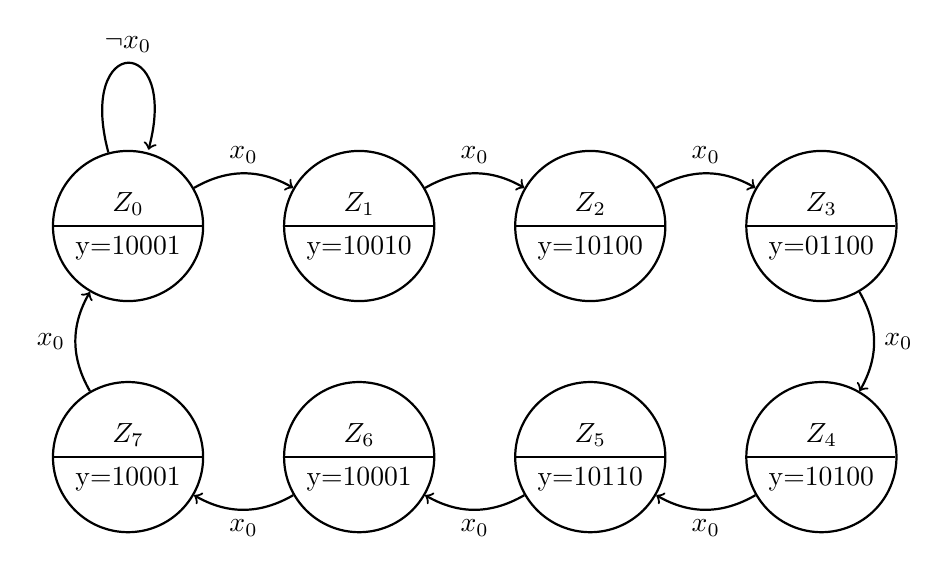
\begin{tikzpicture}[auto,thick]
	\node[state with output] (Z0) {$Z_0$ \nodepart {lower} y=10001};
	\node[state with output, right=of Z0] (Z1) {$Z_1$ \nodepart {lower} y=10010};
	\node[state with output, right=of Z1] (Z2) {$Z_2$ \nodepart {lower} y=10100};
	\node[state with output, right=of Z2] (Z3) {$Z_3$ \nodepart {lower} y=01100};
	\node[state with output, below=of Z3] (Z4) {$Z_4$ \nodepart {lower} y=10100};
	\node[state with output, below=of Z2] (Z5) {$Z_5$ \nodepart {lower} y=10110};
	\node[state with output, below=of Z1] (Z6) {$Z_6$ \nodepart {lower} y=10001};
	\node[state with output, below=of Z0] (Z7) {$Z_7$ \nodepart {lower} y=10001};
	\path[->]
	(Z0)	edge [bend left]	node{$x_0$}	(Z1)
	(Z0)	edge [loop above]			node[swap]{$\neg x_0$}	()
	(Z1)	edge [bend left]	node{$x_0$}	(Z2)
	(Z2)	edge [bend left]	node{$x_0$}	(Z3)
	(Z3)	edge [bend left]	node{$x_0$}	(Z4)
	(Z4)	edge [bend left]	node{$x_0$}	(Z5)
	(Z5)	edge [bend left]	node{$x_0$}	(Z6)
	(Z6)	edge [bend left]	node{$x_0$}	(Z7)
	(Z7)	edge [bend left]	node{$x_0$}	(Z0);
\end{tikzpicture}\\ \\ 
$A=(X,Y,Z, \delta, \mu )$, mit\\
$X=\lbrace 0,1 \rbrace$\\
$Y= \lbrace 10001,10010,10110,01100,10100 \rbrace$\\
$Z=\lbrace 000,001,010,011,100,101,110,111 \rbrace$ \\
$\delta : Z \times X \rightarrow Z$\\
$\mu : Z \rightarrow Y$\\ \\
Die Wertetabelle dazu\\
\begin{tabular}{c | c | c | c | c | | c | c | c | | c | c | c | c | c | c | | c | c | c | c | c}
$x_0$&Z&$z_2$&$z_1$&$z_0$&$z^+_2$&$z^+_1$&$z^+_0$&$J_2$&$K_2$&$J_1$&$K_1$&$J_0$&$K_0$&$y_4$&$y_3$&$y_2$&$y_1$&$y_0$ \\ \hline
0&$Z_0$&0&0&0&0&0&0&0&*&0&*&0&*&1&0&0&0&1\\
0&$Z_1$&0&0&1&0&1&0&0&*&1&*&*&1&1&0&0&0&1\\
0&$Z_2$&0&1&0&0&1&1&0&*&*&0&1&*&1&0&0&0&1\\
0&$Z_3$&0&1&1&1&0&0&1&*&*&1&*&1&1&0&0&0&1\\
0&$Z_4$&1&0&0&1&0&1&*&0&0&*&1&*&1&0&0&0&1\\
0&$Z_5$&1&0&1&1&1&0&*&0&1&*&*&1&1&0&0&1&1\\
0&$Z_6$&1&1&0&1&1&1&*&0&*&0&1&*&1&0&0&0&1\\
0&$Z_7$&1&1&1&0&0&0&*&1&*&1&*&1&1&0&0&0&1\\ \hline
1&$Z_0$&0&0&0&0&0&1&0&*&0&*&1&*&1&0&0&0&1\\
1&$Z_1$&0&0&1&0&1&0&0&*&1&*&*&1&1&0&0&1&0\\
1&$Z_2$&0&1&0&0&1&1&0&*&*&0&1&*&1&0&1&0&0\\
1&$Z_3$&0&1&1&1&0&0&1&*&*&1&*&1&0&1&1&0&0\\
1&$Z_4$&1&0&0&1&0&1&*&0&0&*&1&*&1&0&1&0&0\\
1&$Z_5$&1&0&1&1&1&0&*&0&1&*&*&1&1&0&1&1&0\\
1&$Z_6$&1&1&0&1&1&1&*&0&*&0&1&*&1&0&0&0&1\\
1&$Z_7$&1&1&1&0&0&0&*&1&*&1&*&1&1&0&0&0&1\\
\end{tabular}\\ \\
\karnaughmap{4}{$J_2$}{{$x_0$}{$z_2$}{$z_1$}{$z_0$}}{0001****0001****}{\textcolor{red}{
\put(2,2){\oval(2,2)}}}
$J_2= \textcolor{red}{z_0 \wedge z_1}$
\karnaughmap{4}{$K_2$}{{$x_0$}{$z_2$}{$z_1$}{$z_0$}}{****0001****0001}{\textcolor{red}{
\put(2,2){\oval(2,2)}}}$K_2= \textcolor{red}{z_0 \wedge z_1}$\\\\
\karnaughmap{4}{$J_1$}{{$x_0$}{$z_2$}{$z_1$}{$z_0$}}{01**01**01**01**}{\textcolor{red}{
\put(2,2){\oval(1.9,4)}}}
$J_1= \textcolor{red}{z_0}$
\karnaughmap{4}{$K_1$}{{$z_2$}{$z_1$}{$z_0$}}{**01**01**01**01}{\textcolor{red}{
\put(2,2){\oval(1.9,4)}}}
$K_1= \textcolor{red}{z_0}$\\
\karnaughmap{4}{$J_0$}{{$x_0$}{$z_2$}{$z_1$}{$z_0$}}{0*1*1*1*1*1*1*1*}{
\textcolor{red}{
\put(3,2){\oval(1.9,4)}
}
\textcolor{blue}{
\put(1.75,2){\oval(4,1.9)}
}\textcolor{green}{
\put(1.75,1){\oval(4,1.9)}
}}
$J_0= \textcolor{red}{z_2} \vee \textcolor{blue}{z_1} \vee \textcolor{green}{x_0}$
\karnaughmap{4}{$K_0$}{{$x_0$}{$z_2$}{$z_1$}{$z_0$}}{*1*1*1*1*1*1*1*1}{
\textcolor{red}{
\put(2,2){\oval(4,4)}
}} $K_0= \textcolor{red}{1}$ \\ 
\karnaughmap{3}{$y_4$}{{$z_2$}{$z_1$}{$z_0$}}{11110111}{
\textcolor{red}{
\put(1,1){\oval(2,2)}}
\textcolor{blue}{
\put(1.8,1){\oval(2,2)}}
\textcolor{green}{
\put(2.5,0.5){\oval(1.9,1)}}}$y_4= \textcolor{red}{ \neg z_2} \vee \textcolor{blue}{z_0} \vee \textcolor{green}{(z_1 \wedge z_2)}$\\
\karnaughmap{3}{$y_3$}{{$z_2$}{$z_1$}{$z_0$}}{00001000}{
\textcolor{red}{
\put(3.5,1.5){\oval(1,1)}}}$y_3= \textcolor{red}{ \neg z_0 \wedge \neg z_1 \wedge z_2}$\\
\karnaughmap{3}{$y_2$}{{$z_2$}{$z_1$}{$z_0$}}{00011110}{
\textcolor{red}{
\put(3,1.5){\oval(1.9,1)}}
\textcolor{blue}{
\put(3.25,1){\oval(1,2)}}
\textcolor{green}{
\put(1,0.5){\oval(1,1)}}} $y_2= \textcolor{red}{( \neg z_1 \wedge z_2)} \vee \textcolor{blue}{( \neg z_0 \wedge z_2)} \vee \textcolor{green}{(z_0 \wedge z_1 \wedge \neg z_2)}$\\
\karnaughmap{3}{$y_1$}{{$z_2$}{$z_1$}{$z_0$}}{00100010}{
\textcolor{red}{
\put(0,0.5){\oval(1.9,1)[r]}
\put(4,0.5){\oval(1.9,1)[l]}
}}
$y_1= \textcolor{red}{ \neg z_0 \wedge z_1 }$\\
\karnaughmap{3}{$y_0$}{{$z_2$}{$z_1$}{$z_0$}}{11000001}{
\textcolor{red}{
\put(1,1.5){\oval(2,1)}
}
\textcolor{blue}{
\put(2.3,0.5){\oval(1,0.9)}
}}$y_0= \textcolor{red}{( \neg z_1 \wedge \neg z_2)} \vee \textcolor{blue}{(z_0 \wedge z_1 \wedge z_2)}$

\end{document}
